\chapter{Complementos de Scrum}

Originariamente Scrum no tiene como objetivo dar instrucciones precisas a los equipos sobre la forma concreta en la que deben llevar a cabo su desarrollo. El Scrum propuesto por la Scrum Guide de Scrum.org es bastante simple y básico (ver fig. \ref{fig:Scrum_Flow_basic_ScrumGuide2017}). Con este marco se espera que los equipos hagan lo que sea necesario para ellos, en función de entregar el producto de calidad. Esto significa mejorar Scrum o ir más allá.

Las prácticas y herramientas de desarrollo cambian y mejoran de manera continua y los buenos equipos trabajarán constantemente en pos de obtener el mejor uso de las mismas. Es así como los equipos a medida que maduran agregan ceremonias y actividades necesarias para su contexto conformando un flujo de Scrum Extendido y adaptado a su realidad (ver fig. \ref{fig:Scrum_Flow_Extended-Scrum}). Además, estos equipos adoptan prácticas ágiles e ingenieriles necesarias para desarrollar software de calidad.

Desde esta perspectiva, se puede consensuar un anillo de complementos útiles que rodea al núcleo de Scrum y que pueden potenciar el trabajo ágil y la práctica de ingeniería. Estos complementos son métodos y técnicas complementarias a Scrum, sugerencias y recomendaciones, lecciones aprendidas y conceptos aledaños. En este capítulos trataremos estos temas.

% Malas prácticas, consejos, tecnicas complementarias, casos de estudios

%Técnicas para requerimientos
% Historias de usuarios
% Técnica Killen :  sirve para definir cuales son las cuestiones clave a desarrollar en un proyecto y su priorización logrando un conjunto de historis de usuario.
% Mapas de historia (Técnica propuesta por Jeff Patton)
% Articles: The New User Story Backlog is a Map By Jeff Patton. JPattonAssociates.com, Octuber 8, 2008.
% URL: http://jpattonassociates.com/the-new-backlog/
%Técnicas de Planeación
%Técnicas de estimación
% Poker de planeación
%Técnicas de Comunicación
% Radiadores de información
% Scrum task board
% Comunicación osmótica
% -----------técnica que te permita limitar la cantidad de trabajo en progreso y la priorización de las tareas, como % son la Técnica pomodoro y la Matriz de Eisenhower respectivamente.
%Técnicas de Programación

\newpage
\section{Scrum extendido}

La guía de Scrum propone un marco simple y algo estructurado y, aunque funciona bien como contenedor para otras técnicas, metodologías y prácticas, hacer Scrum es al menos seguir ese marco. Sin embargo, debemos usar lo necesario que en nuestro contexto nos ayude a solucionar los problemas y cumplir los objetivos que nos planteamos. Por tal motivo, debemos ser libres de tomar lo que consideramos relevante de scrum, o mezclarlo con otros métodos o expandirlo con otras ceremonias, técnicas y prácticas.

En mi experiencia he visto como equipos han necesitado robustecer Scrum con otras ceremonias, actividades y procesos como la inception, el refinamiento, demos internas, Monitoreo constante de feedback, proceso de OPCON, break, etcétera. 

\begin{figure}[h]
  \centering
  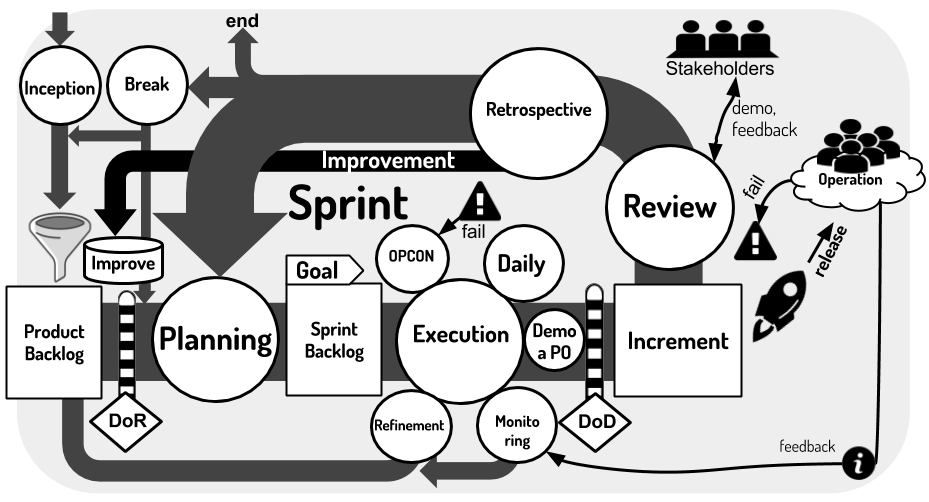
\includegraphics[width=0.99\textwidth]{Scrum_Flow_Extended-Scrum}
  \caption{Flujo de Extended Scrum}
  \centering
  \label{fig:Scrum_Flow_Extended-Scrum} %\ref{fig:Scrum_Flow_Extended-Scrum}
\end{figure}
\FloatBarrier % Command to control the position of floating images. With its, I can get the figures not to be pushed to the end of the document.
% El comando FloatBarrier es usado aqui para que la imagen se clave en este lugar y que no sea acarreada al final del documento.

Por ejemplo, cuando un equipo ya constituido comienza con un nuevo producto, es aconsejable tener un proceso inmediatamente previo a comenzar los sprints para definir o poner a todo el equipo en la misma página respecto a la visión del producto, los objetivos y para poder hacer una primera alimentación formal y colaborativa del backlog. En esta reunión es cuando se hace el kickoff, se definen los tipos de usuarios, experiencia de usuarios a alto nivel, visión del producto, features principales, posibles temas o épicas, un posible roadmap, y las historias sobre las cuales se puede comenzar a trabajar. A este proceso se lo puede llamar “inception”.

Otro ejemplo es el refinamiento o “refinement” que no es una ceremonia oficial de Scrum, sin embargo se puede hacer necesario formalizar el refinamiento como ceremonia para fortalecer el trabajo en equipo sobre el backlog y llegar con historias más maduras (con menos riesgo) a la planning. De hecho, las historias y el DoR no son parte dictada por la guía de Scrum, pero es de bastante utilidad trabajar con historias (como se verá más adelante) y asegurarse de que hay un mutuo entendimiento de la completitud necesaria de una historia para ser abordada en una planning.

También podemos considerar hacer demostraciones “Demo” al PO previas a la review, como instancias donde el equipo junto al PO controlan el DoD y los criterios de aceptación, para controlar una historia antes de que se llegue a la review. De este modo se llega a la review con certeza de cuáles historias se concluyeron satisfactoriamente y cuáles no, evitando que la review se transforme en una instancia de aprobación de historias.

El monitoreo constante de feedback ("Monitoring" o Continuous Monitoring) puede transformarse en un proceso pautado, en el cual el equipo se autogestiona para realizar inspección y adaptación constante, monitoreando las principales métricas del producto, KPIs y registros de actividad del producto funcionando en operaciones. Esto es radicalmente importante para pasar de ser un equipo reactivo a proactivo. Aunque también se debe contemplar ser lo suficientemente efectivo en las acciones reactivas de solución de contingencias en operaciones (resolución de fallos o bugs en operaciones). Y para ello se puede tener un proceso consensuado de cómo manejar las OPCON de forma eficiente.

Trabajar con Scrum se puede sentir, en ocasiones, la disciplina de la cadencia como sofocante. En algunos contextos puede ser producente tener un respiro para que el equipo trabaje en algo fuera del foco del producto o para trabajar en actividades como refinar el backlog, capacitaciones, innovación, planificaciones, teambuilding, discovery, etcétera. Para eso se usa el concepto de “break”, un lapso de tiempo para hacer estas actividades sin contar como sprint. Una especie de interludio inter-sprints.

En síntesis, debemos ser libres de adaptar Scrum o potenciarlo como consideremos apropiado. Ser libres de experimentar.

\subsection{Definición de preparado}

Otro ornamento ya mencionado anteriormente pero no explicado es el "Definition of Ready" o DoR. La definición de preparado es un tipo de Definición de Terminado particular (previo al desarrollo) que, si bien no es parte de la guía de Scrum original, es particularmente útil. Pues, se corresponde con las condiciones para que una historia (PBI) pueda pasar a formar parte de un Sprint Backlog. Si una historia no cumple con su DoR no puede ser tomado en una planificación para ser ítem de trabajo del Sprint planeado, ya que es un ítem que no está suficientemente preparado para ser comprometido para el desarrollo. Es decir necesita refinamiento. O sea que, la definición de preparado permite entonces tener un punto de acuerdo entre el PO y el Equipo, permitiendo conocer cuándo una historia de usuario está realmente lista para evaluar su factibilidad de desarrollo en una reunión de planeamiento y ser llevada a un Sprint.

Un ejemplo de DoR puede ser el que sigue:

\begin{figure}[h]
  \centering
  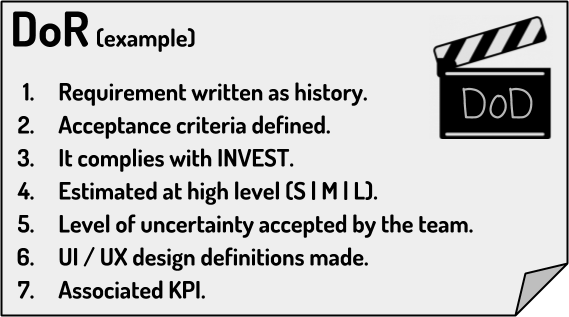
\includegraphics[width=0.60\textwidth]{DoR_example}
  \caption{Ejemplo de una DoR}
  \centering
  \label{fig:DoR_example} %\ref{fig:DoR_example}
\end{figure}
\FloatBarrier % Command to control the position of floating images. With its, I can get the figures not to be pushed to the end of the document.
% El comando FloatBarrier es usado aqui para que la imagen se clave en este lugar y que no sea acarreada al final del documento.



\newpage
\section{Dinámicas de grupo}
\subsection{Coordinar el silencio}

Una técnica usada por rescatistas después de terremotos para hacer silencio es particularmente útil para lograr silencio en un grupo numeroso. Consta de pedir silencio cuando se levanta la mano. Pues, los que ven la mano levantada tienen que callarse y levantar a su vez la mano. Cuando cualquiera ve a alguien con la mano levantada se debe callar y a su vez levantar la mano. Este comportamiento se termina propagando rápidamente en todos los integrantes hasta que se logra el silencio. Es una técnica muy útil en la reuniones cuando las personas se dispersan comunicándose en forma caótica o cuando alguna actividad de conversación libre se extiende del tiempo necesario.

\subsection{Gamification y dinámicas de grupo}

Un facilitador ágil (SM, AM, Agile Coach, etc.) debería facilitar los cambios culturales, la cohesión de equipos, el trabajo colaborativo, la creatividad y la innovación. Para ello, puede traer a la mano, de su cartera de juegos, dinámicas de grupo que son herramientas de Gamification (Game Thinking). Estas dinámicas son actividades en forma de juegos que ayudan a llegar a un resultado grupal de una manera divertida, comprometida, colaborativa, activa, motivadora, visual (Visual Thinking), experimental (Design Thinking) y creativa (Creative Thinking). Hay que considerar que estas dinámicas deben reforzar las actividades de ingeniería y no reemplazarlas.

\subsection{Constitución de un equipo Ágil}

No hay nada mejor para iniciar un equipo ágil que comenzar con motivación, foco y compromiso, para lo cual una dinámica de  “Constitución de un equipo Ágil” es útil. Pues mediante esta técnica se busca lanzar un equipo que tenga identidad como tal, forma de trabajo clara, acuerdos de convivencia, un propósito como foco de equipo y valores que guíen su espíritu. Es una inversión de esfuerzo inicial en un grupo para lograr cohesión, promoviendo su sinergia, para el éxito futuro como equipo. En esta reunión de constitución se recomienda comenzar con alguna dinámica rompe hielo y seguir con una de conocimiento interpersonal, como por ejemplo la dinámica de “mapa personal” (personal map). Luego se puede hacer la dinámica de “Lienzo de Constitución de Equipo Ágil” (ver figura \ref{fig:Lienzo_de_constitucion_de_equipo_agil}). 

\begin{figure}[h]
  \centering
  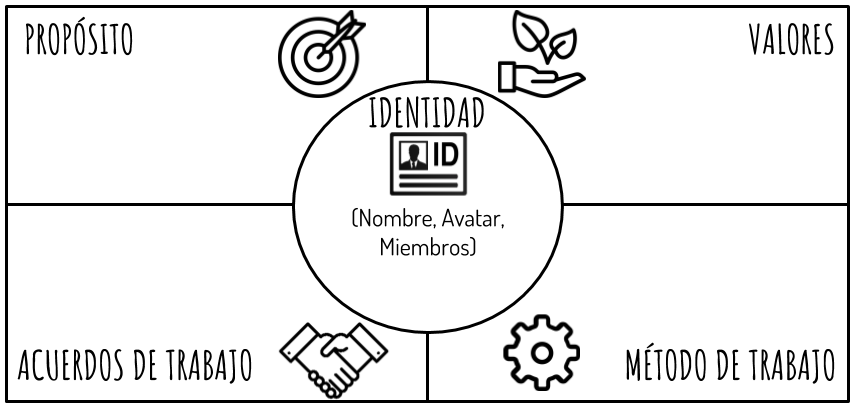
\includegraphics[width=0.99\textwidth]{Lienzo_de_constitucion_de_equipo_agil}
  \caption{Lienzo de Constitución de Equipo Ágil}
  \centering
  \label{fig:Lienzo_de_constitucion_de_equipo_agil} %\ref{fig:Lienzo_de_constitucion_de_equipo_agil}
\end{figure}
\FloatBarrier % Command to control the position of floating images. With its, I can get the figures not to be pushed to the end of the document.
% El comando FloatBarrier es usado aqui para que la imagen se clave en este lugar y que no sea acarreada al final del documento.

En esta dinámica, mediante un lienzo de cinco regiones, completamos la identidad del equipo, su propósito como tal, los valores del equipo, los acuerdos de trabajo (working agreement) y el método de trabajo. La identidad del equipo puede constar de un nombre y un avatar. También se pueden escribir los nombres de cada integrante para que queden registrados como acta de constitución. El propósito debería ser simple y claro, que cohesione la finalidad del equipo. Aquí podemos recordar que es deseable que se constituyan equipos a los cuales se les da trabajo o se les trae productos o proyectos y no al revés, armar equipos para un proyecto en particular para luego desarmarlos. Es recomendable orientarse a productos o servicios con equipos estables que a proyectos. Respecto a los valores, además de hacer énfasis en los valores ágiles y los de Scrum, el equipo puede definir sus propios valores o agregar valores a seguir. Los acuerdos de trabajo son esenciales para marcar las reglas del equipo como acuerdos de convivencia. Aquí se puede agregar la hora de comienzo de la daily, por ejemplo. Y por último, en método de trabajo se aclara el uso de Scrum, la duración del sprint y se pueden especificar algunas prácticas a seguir.

\newpage
\section{Técnicas de justificación de negocio}

\subsection{Retorno de la inversión}

El ROI sirve para estimar el posible valor de Proyecto. Se usa para evaluar los ingresos netos que se esperan obtener a partir de un Proyecto, restando los costos o inversiones estimadas de un Proyecto de su ingreso, y dividiendo esto (beneficio neto) por los costos previstos, con el fin de obtener una tasa de retorno. 

\subsection{Valor de negocio versus complejidad}

Se puede hacer uso de medir Business Value Points para hacer un seguimiento del valor de negocio entregado mediante diagramas de Business Value Delivered (Ver figura \ref{fig:BusinessValueDiagrams}) o Business Value BurnUp\footnote{El Business Value BurnUp es un diagrama de BV entregado acumulado por cada Sprint \cite{Scrum-Alliance-2005}}. Además, también es útil para ayudar en la priorización de historias de usuario, pues logrando hacer un diagrama de Business versus Complexity (Ver figura \ref{fig:BusinessValueDiagrams}) podemos tener una visión del peso en complejidad de cada historia (US) o PBI en contraste con el valor de negocio que aporta y, en base a esto, poder hacer priorizaciones en las sesiones de planificación.

\begin{figure}[h]
  \centering
  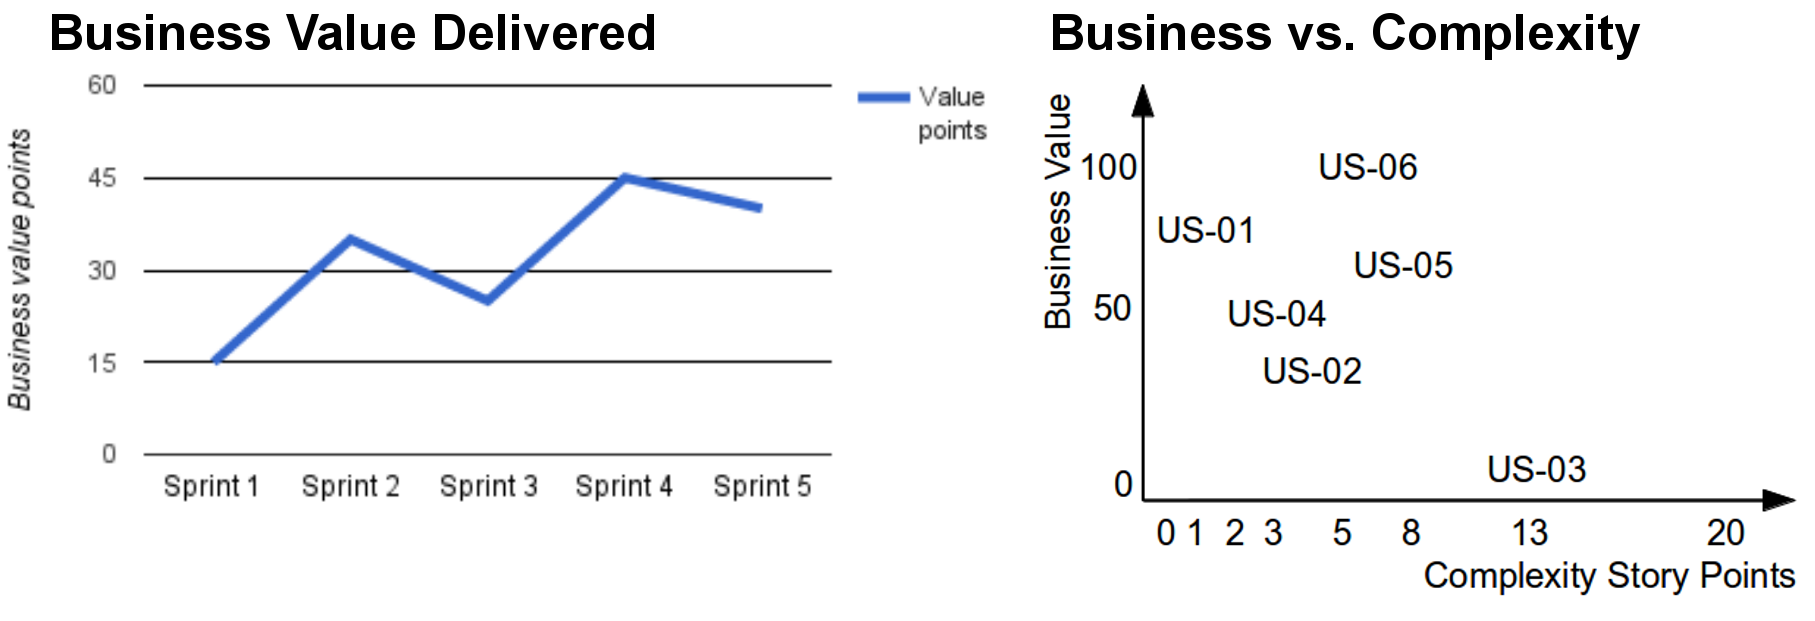
\includegraphics[width=0.99\textwidth]{BusinessValueDiagrams}
  \caption{Diagramas de Business Value}
  \centering
  \label{fig:BusinessValueDiagrams} %\ref{fig:BusinessValueDiagrams}
\end{figure}
\FloatBarrier % Command to control the position of floating images. With its, I can get the figures not to be pushed to the end of the document.
% El comando FloatBarrier es usado aqui para que la imagen se clave en este lugar y que no sea acarreada al final del documento.

\newpage
\section{Técnicas para requerimientos}

\subsection{Historias de usuarios}

Para Scrum las hipótesis de requerimientos se representan en ítems de Backlog de producto PBI. A estos PBIs se los suele denominar "Story" o "Historias de Usuarios"\footnote{Las "User Story" son una técnica de eXtremme Programming (XP)}. El Product Backlog incluye incisos o Stories que aportan valor al cliente y que suelen ser descripción de requisitos funcionales. Aunque también puede incluir entradas para exploración de características, necesidades del cliente u opciones técnicas, requerimientos no funcionales, el trabajo necesario para lanzar el producto, y otros incisos, así como la configuración del entorno o arreglar defectos \footnote{\cite{Scrum-Institute-2015}}. O sea que puede proporcionar valor en forma indirecta mediante el aumento de la calidad o la reducción de los incidentes en el largo plazo \footnote{\cite{Scrum-Institute-2015}}.

Las historias representan un concepto verificable y simple, que el Product Owner quiere implementar en el producto. Según el concepto general de metodología Ágil, la historia se define como una "promesa de una conversación" o una "descripción de una característica" \footnote{\cite{UNTREF-2014}, \cite{Dan-North-2015}}. Según esta perspectiva, la historias de usuario representa una "funcionalidad de aplicación" para un usuario y que brinda un beneficio (ROL + FUNCIONALIDAD + BENEFICIO). Las mismas se escriben siempre con lenguaje de negocio y respetando la siguiente pauta de estructura:\newline

\textbf{COMO} <ROL> \textbf{QUIERO} <FUNCIONALIDAD> \textbf{PARA QUE} <BENEFICIO>\newline

Por ejemplo:
%Example of User Story
\begin{figure}[h]
  \centering
  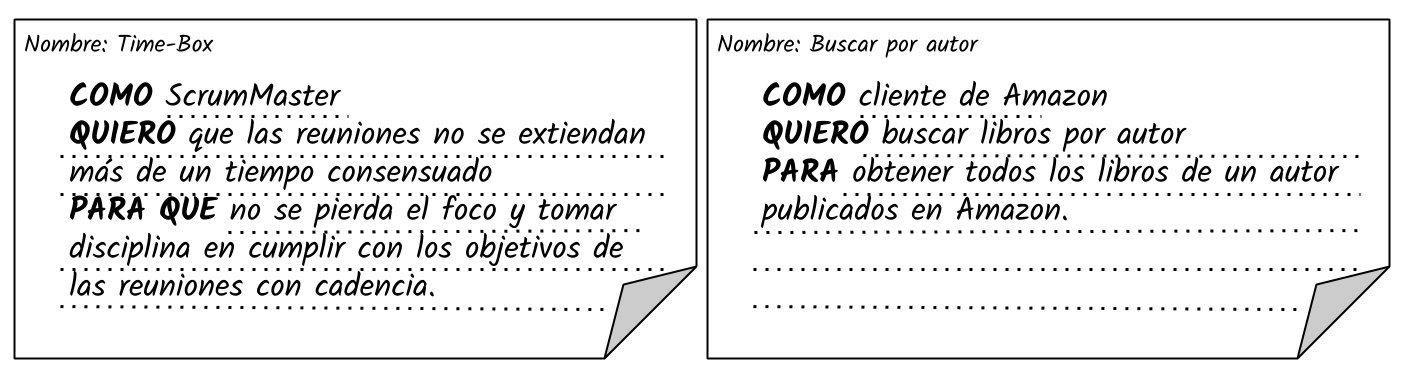
\includegraphics[width=0.99\textwidth]{UserStory_ejemplo}
  \caption{Escritura de historias ejemplo}
  \centering
  \label{fig:StoryHierarchy} %\ref{fig:UserStory_ejemplo}
\end{figure}
\FloatBarrier % Command to control the position of floating images. With its, I can get the figures not to be pushed to the end of the document.
% El comando FloatBarrier es usado aqui para que la imagen se clave en este lugar y que no sea acarreada al final del documento.

La historia de usuario no es exactamente un requerimiento, pero puede considerarse como el título de una hipótesis de requerimiento como recordatorio de algo relevante a conversar con el usuario o cliente. En consecuencia lo relevante es su evolución como conversación \footnote{\cite{UNTREF-2014}}.

La historia de usuario describe lo que el usuario quiere hacer desde la perspectiva de una interacción con un proceso de negocio, describe el objetivo del usuario en términos de necesidad de obtener algo que se hace en el negocio \footnote{\cite{Scott-Bellware-2008}}.

Según Dan North y en el marco de Behavior-Driven Development (BDD), una Story es más un requerimiento, pues tiene que ser una descripción de un requisito y su beneficio para el negocio, y un conjunto de criterios con los que todos estamos de acuerdo de qué es o lo que se hace, "lo que el cliente necesita" \footnote{\cite{Dan-North-2015}}. 

\subsubsection{Criterio de demarcación}

Las historias de usuario bien escritas son esenciales para el desarrollo ágil y la ingeniería de software. Existen ciertas características a tener en cuenta a la hora de escribir una historia de usuario y determinar cuál es una bien escrita o una válida. El criterio de demarcación aceptado en metodología ágil en general es el criterio INVEST\footnote{INVEST es un acrónimo creado por Bill Wake.} y que consta de seis características a cumplir \footnote{\cite{UNTREF-2014}, \cite{Scrum-Alliance-2015}}:

\begin{enumerate}

\item \textbf{Independiente:} una historia debe ser atómica. Es decir que se debe buscar asegurar la cohesión funcional y el bajo acoplamiento entre historias distintas. La fuerte dependencia entre diferentes historias hace que sea más dificil planificar, priorizar y estimar.

\item \textbf{Negociable:} debe ser conversable y en consecuencia negociable (es viva). Las historias "no son requerimientos contractuales"\footnote{"Las user stories no son obligaciones contractuales"\cite{Cohn-2004}} ni requisitos rígidos, y su detalle y precisión debe poder evolucionar en el tiempo en procesos de refinamiento y conversaciones en una ingeniería de requerimientos evolutiva.

\item \textbf{Valuable:} debe generar un valor al cliente (usuario o comprador). Una Story sin una declaración de la motivación del usuario a menudo se piensa que es no accionable; es decir, la historia no se puede estimar o implementar fácilmente \footnote{\cite{Scott-Bellware-2008}}. Lo ideal, además de la declaración explícita del beneficio, es que haya una forma de medir el valor que aporta al cliente.

\item \textbf{Estimable:} se debe poder estimar. La historia debe brindar la suficiente información que de la certidumbre necesaria para que los desarrolladores puedan estimarla y permitir, de este modo, que se pueda priorizar y planificar. 

\item \textbf{Pequeña:} debe ser lo suficientemente pequeña para entrar en un sprint o iteración. El tamaño pequeño de las historias ayuda a reducir el tamaño del lote, incrementar el flujo de valor hacia el cliente y asegurar que cada miembro del equipo de desarrollo pueda hacer una contribución valiosa cada día. Por ejemplo, en cada Sprint se podrían completar entre cuatro y ocho historias pequeñas. A medida que una historia es más grande va a tener más errores asociados a la estimación y alcance, y aumentará la probabilidad de terminar en un Sprint fallido.

\item \textbf{Probable:} debe poder permitir la contrastabilidad. La contrastabilidad del enunciado de la historia es la propiedad de ésta de ser capaz de ser sometida a una prueba empírica y repetible a fin de evaluar su adecuación o no a los hechos a los que se refiere o resultados esperados. Esta característica es crucial para hacer ingeniería, sin la contrastabilidad no se hace ingeniería. Un ejemplo de historia no probable sería: "Como usuario quiero un software hermoso y fácil de usar".

\end{enumerate}

\subsubsection{¿Qué NO es una Historia de Usuario?}

Si no cumple con el criterio INVEST es bastante probable que no sea una User Story. Por ejemplo una tarea puramente técnica (que le interesa sólo al desarrollador), un refactoring técnico, deuda técnica, una mejora técnica o un Spike no cumplen con INVEST y en su generalidad no son User Story. Sin embargo, a todas las historias que no son tareas o spike las podemos tratar como Story, haciendo la distinción entre User Story y Technical Story (ver fig. \ref{fig:StoryHierarchy}).

\begin{figure}[h]
  \centering
  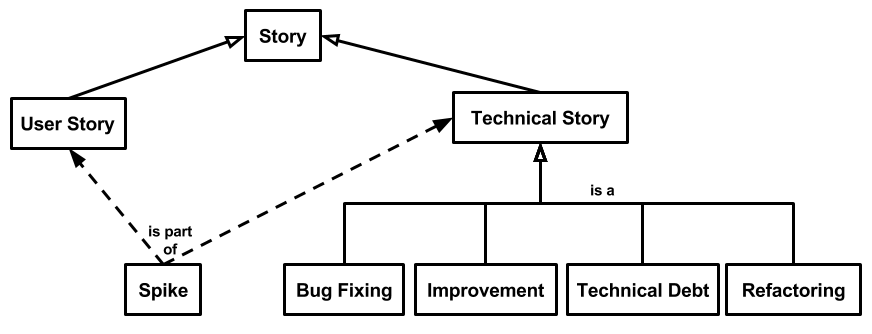
\includegraphics[width=0.99\textwidth]{StoryHierarchy}
  \caption{Clasificación de historias}
  \centering
  \label{fig:StoryHierarchy} %\ref{fig:StoryHierarchy}
\end{figure}

Veamos los siguientes ejemplos:

\begin{itemize}

\item \textbf{Technical Story:}
“Cada historia tiene que ser valorada por los usuarios. Pero eso sería un error."\footnote{\cite{Cohn-2004}} Pues en realidad, una historia de usuario describe la funcionalidad que será valiosa para un usuario o comprador de un sistema o software \footnote{\cite{Cohn-2004}}. Hay historias que especifican aspectos técnicos que no son valiosos para el usuario sino más bien para el cliente o comprador (la valoración es transitiva y no directa). Historias técnicas pueden ser valorados por los compradores que contemplan la compra del producto, pero no serían valorados por los usuarios reales. Pero esto no es lo que podemos llamar una "Technical Story" sino que es una Story con aspectos técnicos que tiene valor para el cliente. Para Scott Ambler, en Agile Modeling, una Story es una definición de muy alto nivel de un requerimiento que puede ser funcional o no, por ejemplo de un requerimiento técnico \footnote{\cite{Scott-Ambler-2015}}, algo así: "\textbf{COMO} usuario \textbf{QUIERO} que las transcripciones estén disponibles en línea a través de un navegador estándar \textbf{PARA QUE} me permita acceder desde cualquier lugar"\footnote{\cite{Scott-Ambler-2015}}.

Cuando se habla de "Technical Story" se referencia a aquella historia técnica que sólo es valorada por los desarrolladores. Estas historias son las que se quieren evitar y considerar como Technical Story que podría ser una tarea técnica, tarea de investigación o tarea por deuda técnica. Este tipo de historias se centran en la tecnología y las ventajas para los programadores. Es muy posible que las ideas detrás de estas historias sean buenas, pero en cambio deben ser escritas para que los beneficios a los clientes o usuarios sean evidentes. Esto permitirá, al cliente, priorizar inteligentemente estas historias en el calendario de desarrollo \footnote{\cite{Cohn-2004}}.

Para la Agile Alliance una Story no se corresponde en general a un "componente técnico" o de la "interfaz de usuario", pues a pesar de que a veces puede ser un atajo útil hablar de por ejemplo "la historia de diálogo de búsqueda", pantallas, cuadros de diálogo y botones, no son historias de usuario \footnote{\cite{Scrum-Alliance-2015}}.

\item \textbf{Spike:}
No es una User Story ya que es una tarea de investigación y/o experimentación en formato time-boxing, por lo que no cumple con ser probable ni estimable (no cumple con dos criterios INVEST); puede ser redactada como una historia de investigación\footnote{\cite{Cohn-2004}}, como por ejemplo: \textbf{COMO} desarrollador \textbf{QUIERO} investigar sobre PERFORMANCE \textbf{PARA QUE} luego se pueda mejorar la prestancia de la aplicación. Un Spike debe ser una tarea corta, preferentemente se trata de que no dure más de 6 horas.\newline

\item \textbf{Refactoring:}
Es una tarea técnica de reingeniería, mejora técnica (Improvement) o deuda técnica (Technical Debt), que no es valuable o su valoración es a futuro o en relación a un atributo de calidad que puede no estar directamente solicitado por el cliente o no impacta en beneficio inmediato para el cliente, ya que podría estar resolviendo una "deuda técnica"\footnote{Deuda técnica es la incurrida involuntariamente debido a trabajos de baja calidad o deuda incurrida intencionalmente (McConnell, Ward Cunningham) y que consta en arquitectura no escalable, defectos en el código, documentación inservible o desactualizada, problemas para migrar o actualizar funcionalidades o problemas por falta de mantenimiento.}. Esto no quiere decir que no pueda haber una "story de refactoring" que puede proporcionar valor en forma indirecta mediante el "aumento de la calidad o la reducción de los incidentes en el largo plazo". Puede ser categorizada como historia técnica.
Un ejemplo es: \textbf{COMO} desarrollador \textbf{QUIERO} hacer un refactory del servicio X \textbf{PARA QUE} se pueda mejorar su arquitectura, lograr código más elegante, más sencillo y asegurar la mantenibilidad de la aplicación.\newline

\item \textbf{Bug Fixing:} La corrección de errores no es una característica nueva de producto, puede deberse a deuda técnica, no ser de valor inmediato para el Dueño de Producto y ser considerada historia técnica. Como estrategia, la misma, puede ser tomada fuera de la carrera (de historias de usuario) del Sprint, es decir, el equipo puede mantener un factor de enfoque en historias de usuario para asegurar tiempo para corregir errores \footnote{\cite{Henrik-Kniberg-2007}}. Hay que tener en cuenta que la corrección de uno o varios errores puede ser tratada simplemente como cualquier otra historia\footnote{\cite{Cohn-2004}} (aunque no sea exactamente una historia de usuario).\newline

\end{itemize}

\subsubsection{Componentes de una historia de usuario}

Las historias de usuarios se componen de tres elementos comunmente denominados las tres 'C'\footnote{Las 3 Cs de Ron Jeffries.}:

\begin{enumerate}

\item \textbf{Carta o tarjeta (Card):} Las historias se deben poder escribir en una tarjeta de papel pequeña. Por ese motivo la redacción de las mismas debe ser clara, precisa y concisa para caber en una tarjeta de papel.

\item \textbf{Conversación:} Las historias deben tener y generar conversaciones cara a cara entre el Product Owner y el Equipo de Desarrollo.

\item \textbf{Confirmación:} Deben estar suficientemente explicada para que el Equipo de Desarrollo qué es lo que se desea construir y qué es lo que se espera como resultado de dicha implementación. La confirmación es el "Criterio de Aceptación" que los desarrolladores deben tener en cuenta para que la misma sea aceptada por el cliente.

\end{enumerate}

\subsubsection{Criterio de aceptación}

Las historias de usuario tienen límites específicos para las características del producto, proceso o servicio definido en la hipótesis de requerimiento que determinan los resultados esperados para que la historia sea aceptada por el cliente. En otras palabras, el criterio de aceptación es el conjunto de afirmaciones útiles para que el cliente valide la historia.

\begin{figure}[h]
  \centering
  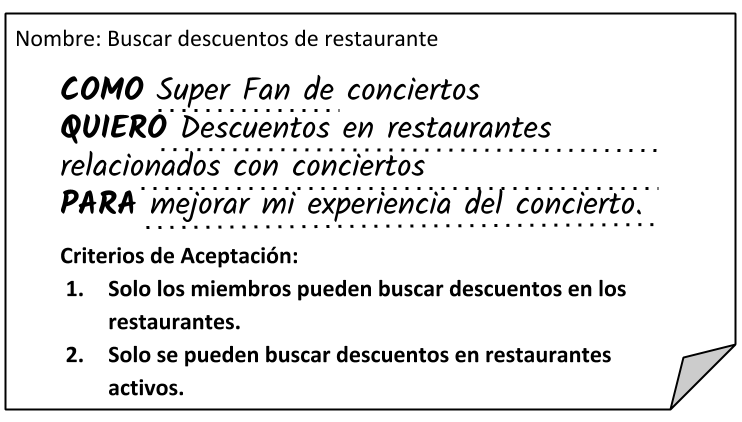
\includegraphics[width=0.70\textwidth]{UserStory_with_CA}
  \caption{Historia de usuario como ejemplo simple}
  \centering
  \label{fig:UserStory_with_CA} %\ref{fig:UserStory_with_CA}
\end{figure}
\FloatBarrier % Command to control the position of floating images. With its, I can get the figures not to be pushed to the end of the document.
% El comando FloatBarrier es usado aqui para que la imagen se clave en este lugar y que no sea acarreada al final del documento.

La estructura de un criterio de aceptación presentado como escenario puede ser como la siguiente:

%Criterio de aceptación ejemplo con un escenario
\begin{itemize}
\item \textbf{Scenario 1:} Título
  \begin{itemize}
  \item \textbf{Given} [contexto] And [otro contexto]...
  \item \textbf{When}  [evento] 
  \item \textbf{Then}  [resultado] And [otro resultado]...
  \end{itemize}
\end{itemize}

\subsubsection{Jerarquía en el backlog}

Una decisión importante a la hora de trabajar con historias de usuario es hacer la estricta demarcación o no. La primera opción es ser estrictos y categorizarlas según si son historias de usuario o técnicas y, de este modo, podemos medir la velocity sobre historias reales y el capacity en trabajo técnico. También visualmente nos da una idea del balance de trabajo técnico versus historias de cara al usuario. Esto requiere más detalle y disciplina. La otra opción es tratarlas a todas como historias. De este modo podremos darnos cuenta si son técnicas o no según el rol que figure en el “COMO” de la redacción. Lo que sí es conveniente es redactar a todas con el formato de historia.
Otras categorías a tener en cuenta son las abstracciones de alto nivel como son: los temas (theme) y las épicas (epic). Hacer este tipo de categorizaciones nos ayudará a hacer mejor el desglose de trabajo y ordenar mejor el backlog. De este modo, podremos agrupar por niveles desde temas en el superior, épicas que agrupan historias y las historias que agrupan tareas (ver fig. \ref{fig:Jerarquias_en_backlog}). Otra manera de agrupar sin usar épicas ni temas es simplemente agrupar por MVPs. Esto dependerá del equipo y el PO, de lo que les sea más cómodo y útil.

\begin{figure}[h]
  \centering
  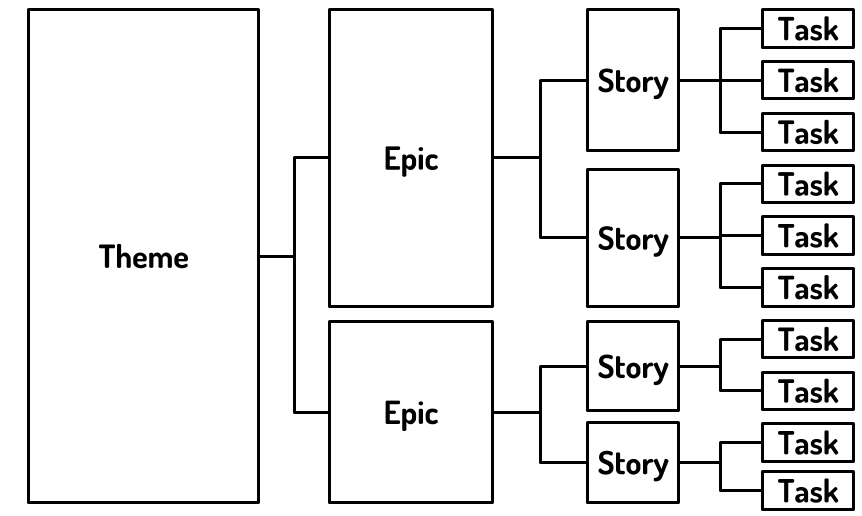
\includegraphics[width=0.8\textwidth]{Jerarquias_en_backlog}
  \caption{Jerarquía en el backlog.}
  \centering
  \label{fig:Jerarquias_en_backlog} %\ref{fig:Jerarquias_en_backlog}
\end{figure}

\subsection{BDD}

Una manera de ayudar al desarrollo ágil a partir de requerimientos es usar el desarrollo conducido por comportamiento (Behavior Driven Development o BDD), el cual es un proceso de desarrollo por el que se busca comenzar a partir de un lenguaje común que une la parte técnica y la de negocio, y desde ese lenguaje común se parte hacia el Testing y, posteriormente, al desarrollo. El proceso consta básicamente en escribir las historias de usuario o features (en lenguaje ubicuo), escribir los escenarios (o criterios de aceptación en forma de escenarios) y automatizar las pruebas de aceptación de los escenarios (aquí es donde comenzamos a hacer TDD).


\section{Técnicas de estimación}

El desarrollo de software es una actividad de creación por evolución del conocimiento y, bajo el marco ágil, esta evolución es adaptativa, produciendo valor en lotes pequeños de trabajo. Esto hace que las planificaciones adaptativas sean más a corto plazo, donde las estimaciones de esfuerzo son realizadas con frecuencia para estimar iteraciones y conversar. 

\begin{figure}[h]
  \centering
  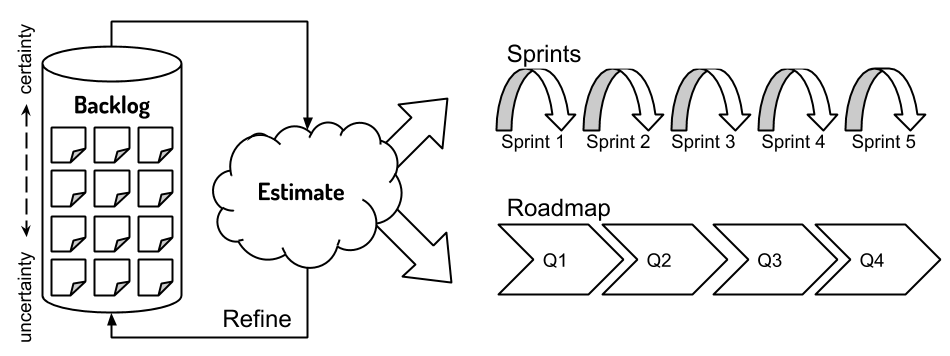
\includegraphics[width=0.9\textwidth]{Estimate}
  \caption{Estimación}
  \centering
  \label{fig:Estimate} %\ref{fig:Estimate}
\end{figure}
\FloatBarrier % Command to control the position of floating images. With its, I can get the figures not to be pushed to the end of the document.
% El comando FloatBarrier es usado aqui para que la imagen se clave en este lugar y que no sea acarreada al final del documento.

Hay que considerar, entonces, que bajo el marco Scrum las estimaciones se hacen con dos razones principales: planificar sprints (sprints, roadmap, etc.) y evolucionar el conocimiento compartido (refinando las historias). La primera está relacionada a la predictibilidad del trabajo en pos de lograr una cadencia sostenible. En este aspecto, la predictibilidad se hace más certera al aumentar el grado de confianza al trabajar con sprint y hacer estimaciones a corta distancia en el tiempo. Además, es parte de un mecanismo de autoregulación del equipo en buscar lograr un flujo de trabajo sostenible, estable y homogéneo. Para ello, el equipo busca desglosar trabajo en esfuerzos equiparables y de tamaños similares. La segunda razón, que se puede considerar la principal para estimar, es la de evolucionar el conocimiento compartido en forma colaborativa. El tiempo insumido en estimar es tiempo aprovechado para charlar en equipo, generando entendimiento común en lo que se tiene que hacer y cómo hay que hacerlo. Si bien el entendimiento común se va madurando en los refinamientos, donde se pueden hacer etimaciones a alto nivel, es en la planning cuando se valida que todos están en la misma página y, desde esta perspectiva, es una excusa para conversar. A continuación comento algunas técnicas elementales.

\subsection{Estimación relativa}

¿Para cuándo va a estar el desarrollo terminado? ¿Cuántas horas vas a demorar en terminar la historia? No queremos estimar en tiempo absoluto, porque estimar cuánto nos vamos a demorar en desarrollar una historia de software, es tan imposible como estimar cuánto dinero exacto vamos a ganar con esa historia. Debido a la complejidad inherente al desarrollo de software es que se recomienda la estimación relativa y que consiste en estimar bajo determinada incertidumbre y con valores relativos. Se suelen usar los puntos de historia o "Story Points", que son una medida relativa de estimación de un ítem de trabajo o una historia de usuario para poder medir su tamaño y, además, es útil para medir la velocidad de un equipo. Hacer estimaciones relativas con SP significa que las historias se comparan entre sí, buscando mantener una relación proporcional entre ellas según estos puntos de historia. O sea que si se piensa a nivel de esfuerzo, una historia que tiene 3 puntos de historia requerirá tres veces más de esfuerzo que una que sea de un punto historia.

\begin{figure}[h]
  \centering
  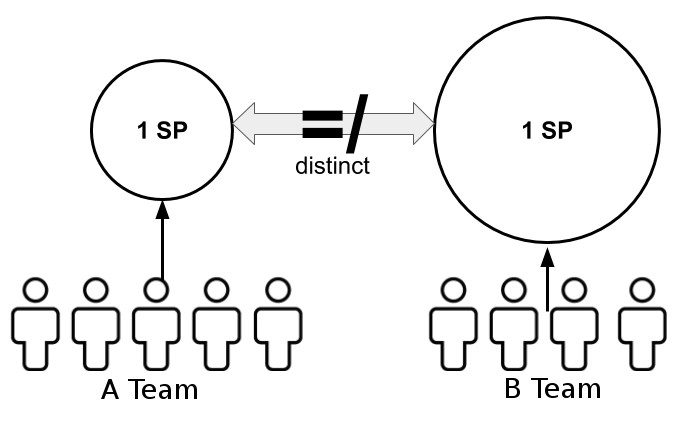
\includegraphics[width=0.6\textwidth]{Storypoints_between_teams}
  \caption{Estimación relativa}
  \centering
  \label{fig:Storypoints_between_teams} %\ref{fig:Storypoints_between_teams}
\end{figure}
\FloatBarrier % Command to control the position of floating images. With its, I can get the figures not to be pushed to the end of the document.
% El comando FloatBarrier es usado aqui para que la imagen se clave en este lugar y que no sea acarreada al final del documento.


Cabe recalcar que la estimación es relativa, porque es subjetiva al equipo que estima. Entonces, si diferentes equipos toman a los puntos de historia como medida de complejidad de una historia, pueden llegar a valores distintos, porque considerarán la complejidad acorde a su percepción de complejidad y que es diferente. Hay equipos que pueden tomar al SP como expectativa de esfuerzo en un día ideal de trabajo (día sin impedimentos) y la expectativa de esfuerzo resultará relativa al equipo que la forma\footnote{\cite{Cohn-2004}}.

También cabe aclarar que "bajo ningún punto de vista la estimación (en story points) es un compromiso"\footnote{\cite{UNTREF-2014}} y que los puntos de historia no son medidas objetivas convertibles en forma precisa a horas. Justamente se usan puntos de historia para no estimar en horas hombre. 

\subsection{Poker de planeación}

El Poker de planeación o "Planning Poker"\footnote{El "Planning Poker" proviene de un paper presentado por James Greening llamado "cómo evitar análisis parálisis en la planificación de liberaciones"\cite{James-Grenning-2002} donde se basa en el método Wideband Delphi para realizar la estimación de requerimientos de forma colaborativa. Luego el método fue popularizado por Mike Cohn con su libro "Agile Estimating and Planning"\cite{Cohn-2005}} es una técnica de estimación y planificación ágil que se basa el consenso por sabiduría de grupo. 

La dinámica consiste en que el Product Owner inicia leyendo una historia de usuario ágil o describe una característica para los desarrolladores estimadores. Cada estimador posee una baraja de "Cartas de Poker de Planificación". Los valores representan el número de puntos de la historia, día ideal, u otras unidades en las que el equipo estima. Los estimadores discutir la función, haciendo preguntas al Product Owner, según sea necesario. Cuando la función se ha discutido plenamente, cada estimador selecciona de forma privada una tarjeta a representar a su estimación. Todas las tarjetas se revelaron a continuación, al mismo tiempo. Si todos los estimadores seleccionan el mismo valor, que se convierte en la estimación. Si no, los estimadores discuten sus estimaciones. Los estimadores de valores altos y bajos deben compartir sus razones. Tras un nuevo debate, cada estimador vuelve a seleccionar una tarjeta de estimación, y todas las tarjetas se revelan de nuevo al mismo tiempo. El proceso se repite hasta que se logre el consenso, o hasta que los estimadores deciden que la estimación ágil y planificación de un ítem en particular debe ser diferida hasta que la información adicional se puede adquirir.


\subsubsection{Cartas de estimación}

Las Cartas de Poker de Planificación que más se usan son las T-Shirts y las de Fibonacci:

\begin{enumerate}

\item \textbf{T-Shirts:} Las cartas de talles de camisetas (polera) contempla los valores XS (muy pequeño), S (Pequeño), M (Mediano), L (grande), XL (muy grande) y XXL (extra grande). En su forma más simple se puede usar: S, M y L. Estos valores sirven para estimar épicas, tamaños de historias o trabajo a alto nivel como el tamaño de funcionalidades. Este tipo de estimación se suele usar en los refinamientos del backlog y nos puede sugerir que una historia es lo bastante grande como para considerar desglosarla (Story Slicing) o lo suficientemente pequeña para tomarla en un futuro sprint.

\item \textbf{Fibonacci:} Las cartas Fibonacci modificada contempla los valores 0, 1, 2, 3, 5, 8, 13, 20, 40 y 100, que se basa en la secuencia fibonacci que se suele recomendar. Estos valores son útiles para estimar complejidad de historias o trabajo a nivel medio. Realizando una estimación relativa, estos valores corresponden a puntos de historia con los que se puede pesar un ítem de trabajo. Este tipo de estimación se suele usar en el planeamiento del sprint para estimar cuántas historias abordar.

\end{enumerate}

\newpage
\section{Técnicas de monitoreo visual}

Para buscar la adaptación y que el equipo se autoregule, debe monitorear constantemente su trabajo y sus resultados. Aquí se muestran algunas herramientas de monitoreo visual.

\subsection{Gestión visual}

La gestión visual es la utilización de elementos y técnicas visuales, como complemento, para la organización del trabajo y la comunicación o irradiación visual del trabajo. Esto es útil para soporte de coordinación y comunicación del equipo y para brindar transparencia hacia interesados externos al equipo.
Es aconsejable que los irradiadores de información presenten las siguientes características:

\begin{enumerate}

\item \textbf{Ubicación ostensible:} estar ubicado en el lugar de trabajo en paredes o paneles visibles para todo el equipo.

\item \textbf{Soporte físico:} estar hechos de material tangible como papel en vez de usar software, salvo el caso de monitores grandes. Por ejemplo en forma de afiches (flip-chart), carteles o pizarras visibles.

\item \textbf{Resumen autoexplicativo:} contener información importante autoexplicativa y didáctica.

\end{enumerate}

Ejemplos de irradiadores de información son: tablero de obstáculos o impedimentos, los gráficos de esfuerzo pendiente burndown y burnup, el gráfico de velocidad, indicadores de estados del build (usando semáforos), métricas de errores, riesgos activos, etcétera.

\subsection{Tableros Scrum/Kanban}

El tablero Scrum/Kanban o "Scrum Kanban Board" es una técnica de comunicación y monitoreo que consiste en utilizar un tablero Kanban (ver figura \ref{fig:ScrumKanbanBoard}), como irradiador de información, para el manejo del ciclo de estados de las tareas y de los impedimentos. El tablero Kanban debe ser visible por todo el equipo y, por lo tanto, transparente para todos los involucrados. Por ejemplo, durante una Daily Scrum todo el equipo es capaz de ver qué tareas se resuelven, cuáles no se han abordado todavía y qué impedimentos existen.

\subsubsection{Ejemplo de un Scrum kanban board}

Los tableros se usan para reflejar el sprint backlog de una manera que sea útil para el equipo. Un buen tablero refleja el flujo real de trabajo y los respectivos WIP asociados a las etapas de trabajo (columnas). Hay equipos que tienen dos tableros: uno para el flujo de historias (story board) y otro para el flujo de las tareas (task board) (ver fig. \ref{fig:SprintBoard_01}). Esta manera permite tener una verdadera visibilidad del flujo de las historias, por un lado, y sus correspondientes tareas, por otro. Otros equipos tienen las historias y tareas integradas en un solo tablero (ver fig. \ref{fig:StoryAndTaskBoard_integrated_01}). La estructura y estándar de colores y nomenclaturas dependerá de cada equipo.

\begin{figure}[h]
  \centering
  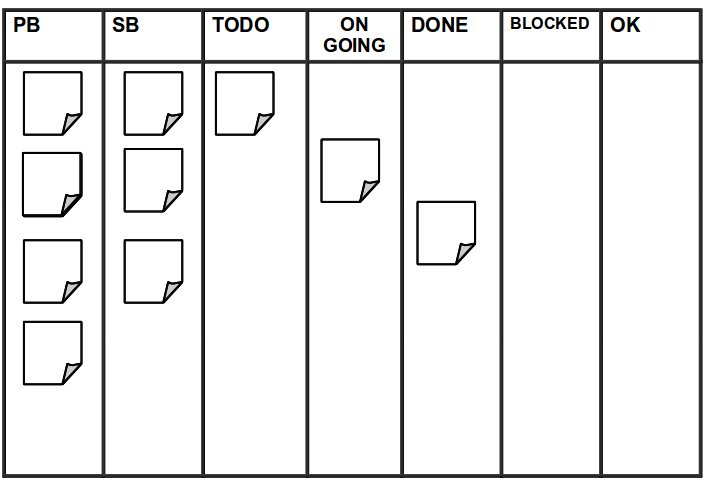
\includegraphics[width=0.8\textwidth]{ScrumKanbanBoard}
  \caption{Ejemplo de un tablero Kanban para Scrum.}
  \centering
  \label{fig:ScrumKanbanBoard} %\ref{fig:ScrumKanbanBoard}
\end{figure}
\FloatBarrier % Command to control the position of floating images. With its, I can get the figures not to be pushed to the end of the document.
% El comando FloatBarrier es usado aqui para que la imagen se clave en este lugar y que no sea acarreada al final del documento.

\begin{figure}[h]
  \centering
  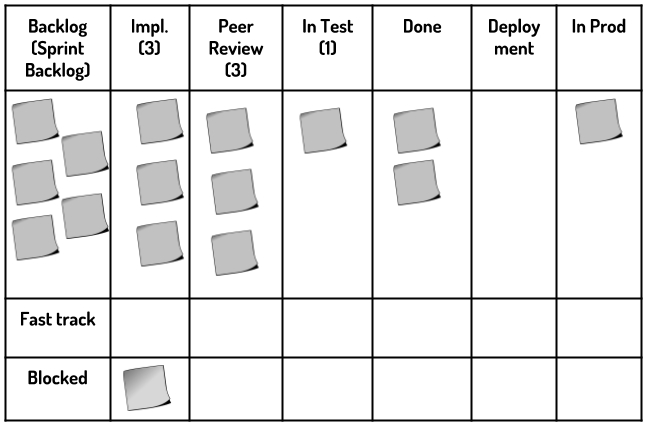
\includegraphics[width=0.8\textwidth]{StoryBoard_01}
  \caption{Ejemplo de un tablero Kanban para historias.}
  \centering
  \label{fig:StoryBoard_01} %\ref{fig:StoryBoard_01}
\end{figure}
\FloatBarrier % Command to control the position of floating images. With its, I can get the figures not to be pushed to the end of the document.
% El comando FloatBarrier es usado aqui para que la imagen se clave en este lugar y que no sea acarreada al final del documento.

\begin{figure}[h]
  \centering
  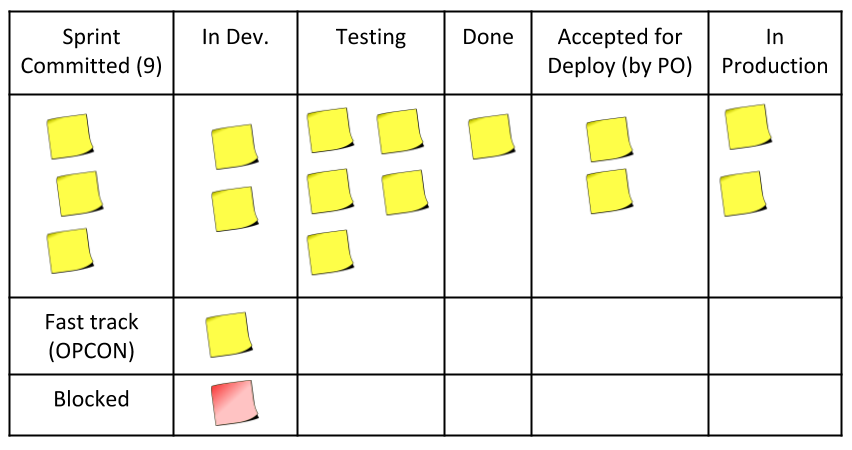
\includegraphics[width=0.9\textwidth]{Kanban_Board_Sierra-India-LATAM-Airlines}
  \caption{Ejemplo de un tablero Kanban físico que usamos con un equipo (Sierra India) en LATAM Airlines.}
  \centering
  \label{fig:Kanban_Board_Sierra-India-LATAM-Airlines} %\ref{fig:Kanban_Board_Sierra-India-LATAM-Airlines}
\end{figure}
\FloatBarrier % Command to control the position of floating images. With its, I can get the figures not to be pushed to the end of the document.
% El comando FloatBarrier es usado aqui para que la imagen se clave en este lugar y que no sea acarreada al final del documento.


\begin{figure}[h]
  \centering
  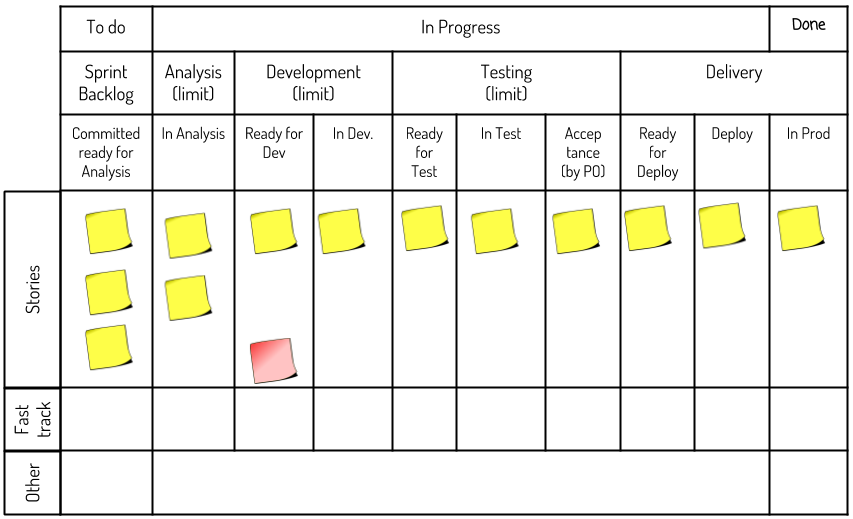
\includegraphics[width=0.99\textwidth]{KanbanBoard_to_Scrum_complex_01}
  \caption{Ejemplo de un tablero Kanban para Scrum sofisticado.}
  \centering
  \label{fig:KanbanBoard_to_Scrum_complex_01} %\ref{fig:KanbanBoard_to_Scrum_complex_01}
\end{figure}
\FloatBarrier % Command to control the position of floating images. With its, I can get the figures not to be pushed to the end of the document.
% El comando FloatBarrier es usado aqui para que la imagen se clave en este lugar y que no sea acarreada al final del documento.

\begin{figure}[h]
  \centering
  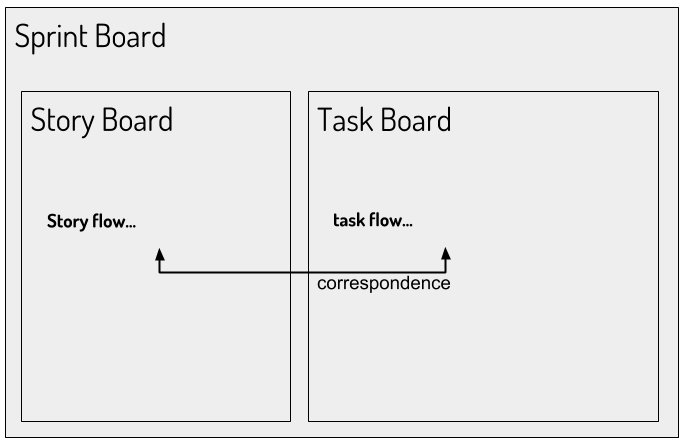
\includegraphics[width=0.8\textwidth]{SprintBoard_01}
  \caption{Esquema de un Sprint backlog.}
  \centering
  \label{fig:SprintBoard_01} %\ref{fig:SprintBoard_01}
\end{figure}
\FloatBarrier % Command to control the position of floating images. With its, I can get the figures not to be pushed to the end of the document.
% El comando FloatBarrier es usado aqui para que la imagen se clave en este lugar y que no sea acarreada al final del documento.


\begin{figure}[h]
  \centering
  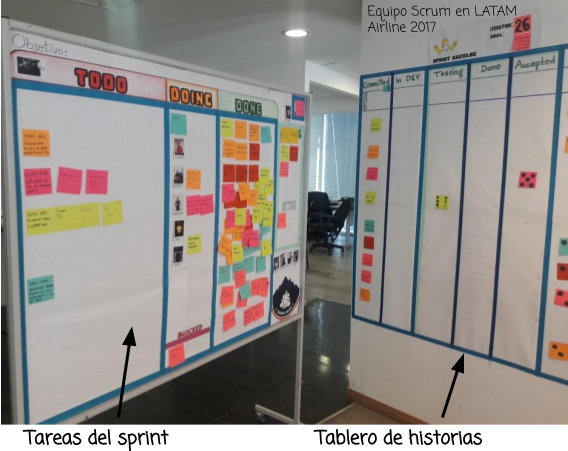
\includegraphics[width=0.99\textwidth]{Tableros_SierraIndia}
  \caption{Ejeplo de tableros físicos en LATAM Airlines 2017.}
  \centering
  \label{fig:Tableros_SierraIndia} %\ref{fig:Tableros_SierraIndia}
\end{figure}
\FloatBarrier % Command to control the position of floating images. With its, I can get the figures not to be pushed to the end of the document.
% El comando FloatBarrier es usado aqui para que la imagen se clave en este lugar y que no sea acarreada al final del documento.



\subsubsection{Ejemplo de un sprint backlog integrado simple}

Un tablero de tareas (taskboard) físico (Ver figura \ref{fig:StoryAndTaskBoard_integrated_01}) es una tabla donde se colocan Post-its representando tareas, que pueden estar asociadas a historias. Este se puede integrar al de historias aunque simplifica el flujo real de la historia ya que se centra en las tareas (ver fig. \ref{fig:StoryAndTaskBoard_integrated_01}).

\begin{figure}[h]
  \centering
  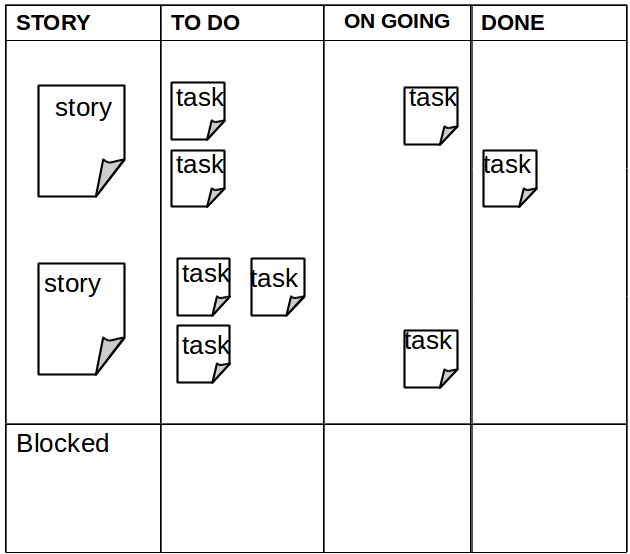
\includegraphics[width=0.6\textwidth]{StoryAndTaskBoard_integrated_01}
  \caption{Ejemplo de un tablero integrado de historia y tareas.}
  \centering
  \label{fig:StoryAndTaskBoard_integrated_01} %\ref{fig:StoryAndTaskBoard_integrated_01}
\end{figure}
\FloatBarrier % Command to control the position of floating images. With its, I can get the figures not to be pushed to the end of the document.
% El comando FloatBarrier es usado aqui para que la imagen se clave en este lugar y que no sea acarreada al final del documento.

\subsection{Tablero de obstáculos}

El Tablero de Obstáculos (ver figura \ref{fig:ObstacleBoard}) es una herramienta visual útil para hacer seguimiento de los obstáculos o bloqueos del equipo que surgen en el trabajo del Sprint. El dueño del Tablero de Obstáculos es el Scrum Master, quien se encarga de buscar o facilitar remover todos los obstáculos que puedan paralizar o ralentizar el trabajo del equipo o desviarlo de su foco esencial. El tablero también es útil para tener la visibilidad del estado de los obstáculos (ver figura \ref{fig:ObstacleBoard}).

\begin{figure}[h]
  \centering
  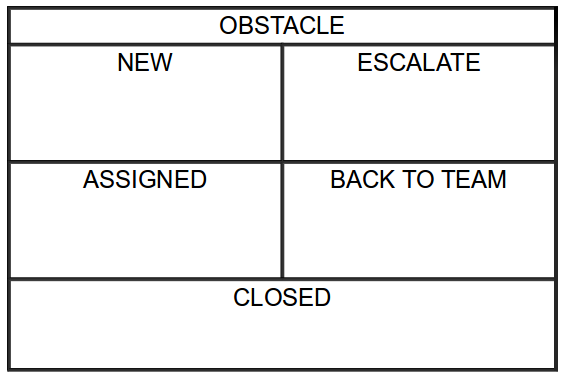
\includegraphics[width=0.6\textwidth]{ObstacleBoard}
  \caption{Ejemplo de un tablero de Obstáculos.}
  \centering
  \label{fig:ObstacleBoard} %\ref{fig:ObstacleBoard}
\end{figure}
\FloatBarrier % Command to control the position of floating images. With its, I can get the figures not to be pushed to the end of the document.
% El comando FloatBarrier es usado aqui para que la imagen se clave en este lugar y que no sea acarreada al final del documento.

\subsection{Calendario de obstáculos}

El calendario de obstáculos es una herramienta visual útil para mostrar los problemas surgidos en todos los sprints hasta el momento (ver figura \ref{fig:CalendarIssues}.).

\begin{figure}[h]
  \centering
  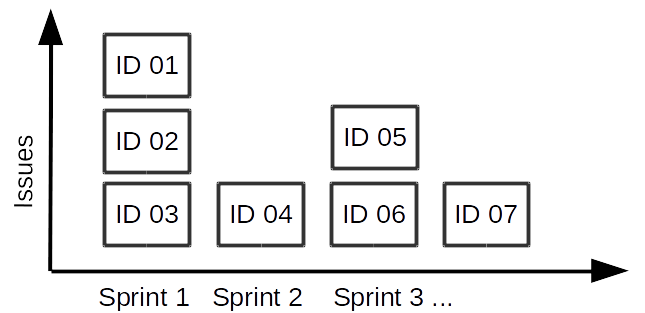
\includegraphics[width=0.6\textwidth]{CalendarIssues}
  \caption{Calendario de obstáculos ejemplo.}
  \centering
  \label{fig:CalendarIssues} %\ref{fig:CalendarIssues}
\end{figure}
\FloatBarrier % Command to control the position of floating images. With its, I can get the figures not to be pushed to the end of the document.
% El comando FloatBarrier es usado aqui para que la imagen se clave en este lugar y que no sea acarreada al final del documento.

\subsection{Gráficos de esfuerzo pendiente}

\subsubsection{Gráfico Burndown}

Un gráfico de trabajo pendiente o "Burndown charts"\footnote{El Burndown muestra la cantidad de trabajo que queda. \cite{SBOK-2013}} (figura \ref{fig:Burndown_chart}) es una técnica de monitoreo para la auto-regulación que muestra el trabajo restante ("Remaining Scope") o que queda por hacer versus tiempo. También refleja la velocidad a la que se están completando los PBIs o historias reflejando el avance y permitiendo extrapolar si el equipo podrá completar el trabajo en el tiempo restante.

\begin{figure}[h]
  \centering
  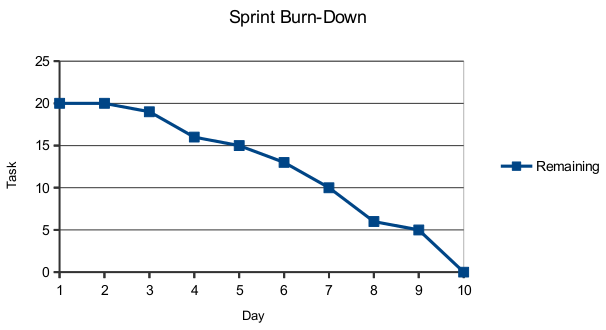
\includegraphics[width=0.9\textwidth]{Burndown_chart}
  \caption{Ejemplo de un gráfico Burndown con un sprint de dos semanas y 20 tareas comprometidas.}
  \centering
  \label{fig:Burndown_chart} %\ref{fig:Burndown_chart}
\end{figure}
\FloatBarrier % Command to control the position of floating images. With its, I can get the figures not to be pushed to the end of the document.
% El comando FloatBarrier es usado aqui para que la imagen se clave en este lugar y que no sea acarreada al final del documento.

\begin{figure}[h]
  \centering
  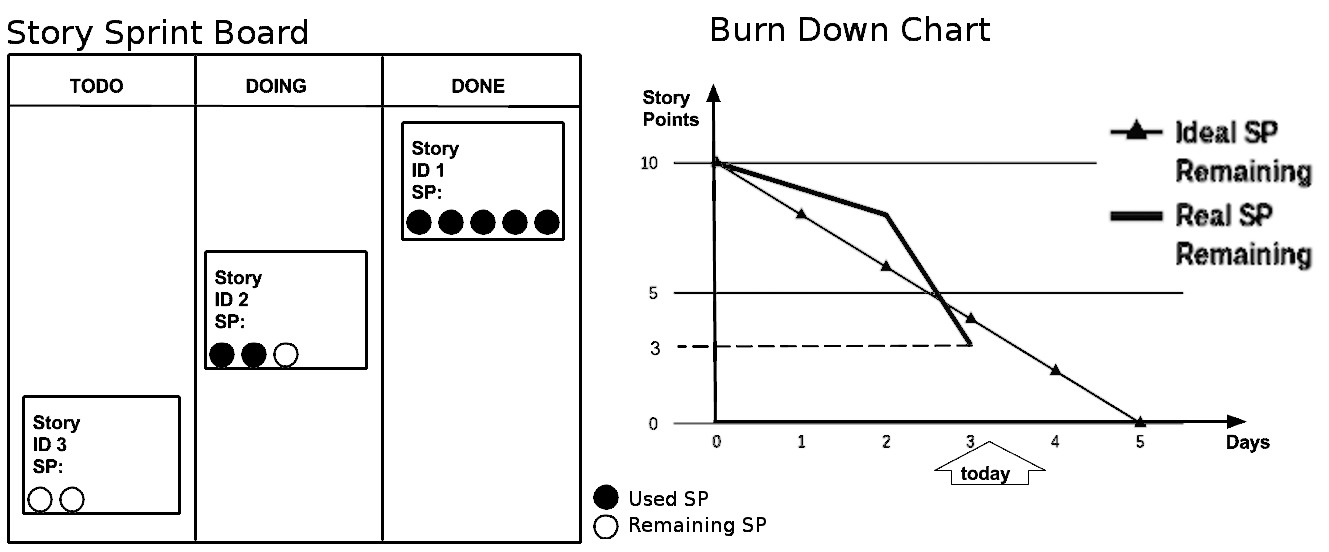
\includegraphics[width=0.99\textwidth]{Burndown-chart_example}
  \caption{Ejemplo de cómo llevar un Burndown con un sprint de 5 días y quedando 3 storypoints por quemar.}
  \centering
  \label{fig:Burndown-chart_example} %\ref{fig:Burndown-chart_example}
\end{figure}
\FloatBarrier % Command to control the position of floating images. With its, I can get the figures not to be pushed to the end of the document.
% El comando FloatBarrier es usado aqui para que la imagen se clave en este lugar y que no sea acarreada al final del documento.

Se pueden utilizan dos gráficos de esfuerzo pendiente:

\begin{enumerate}

\item \textbf{Burndown de Sprint:} Días u horas pendientes para completar las tareas de la iteración (sprint burndown chart), realizado a partir de la lista de tareas o historias de la iteración. Normalmente se utiliza para saber cuánto falta para terminar las historias comprometidas en un Sprint. Es un diagrama de dos ejes: en el eje X el tiempo en días de duración del sprint, en el eje Y la cantidad de trabajo comprometido con el cliente durante el sprint en las unidades que se hayan acordado, story points o tareas (ver figuras \ref{fig:Burndown_chart} y \ref{fig:Burndown-chart_example}).

\item \textbf{Burndown de Proyecto:} Días pendientes para completar los requisitos del producto o proyecto (product burndown chart), realizado a partir de la lista de requisitos priorizada (Product Backlog).

\end{enumerate}

\subsubsection{Gráfico Burn-Up}

El gráfico de trabajo realizado o Burn-up\footnote{El Burnup muestra el trabajo realizado como parte de la Sprint. \cite{SBOK-2013}} (figura \ref{fig:Burnup_chart}) es muy similar al Burndown, con la diferencia de que se parte del cero, y se va marcando la cantidad de trabajo completado en el Sprint. En este gráfico la curva va hacia arriba acercándose a una línea que representa el alcance comprometido. En este tipo de gráfico es más fácil visualizar los cambios de alcance y ver la diferencia entre estimado y real (ver \ref{fig:Burnup-chart_example}).

\begin{figure}[h]
  \centering
  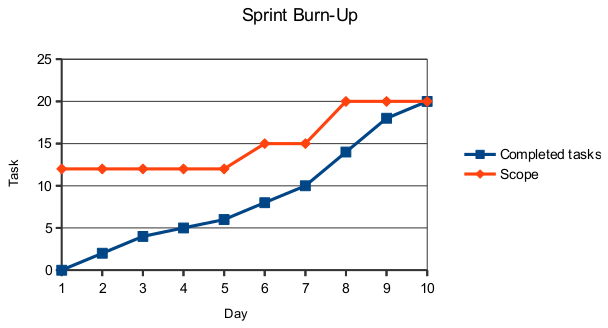
\includegraphics[width=0.85\textwidth]{Burnup_chart}
  \caption{Ejemplo de un gráfico Burnup de tareas comprometidas en un sprint de dos semanas.}
  \centering
  \label{fig:Burnup_chart} %\ref{fig:Burnup_chart}
\end{figure}
\FloatBarrier % Command to control the position of floating images. With its, I can get the figures not to be pushed to the end of the document.
% El comando FloatBarrier es usado aqui para que la imagen se clave en este lugar y que no sea acarreada al final del documento.

\begin{figure}[h]
  \centering
  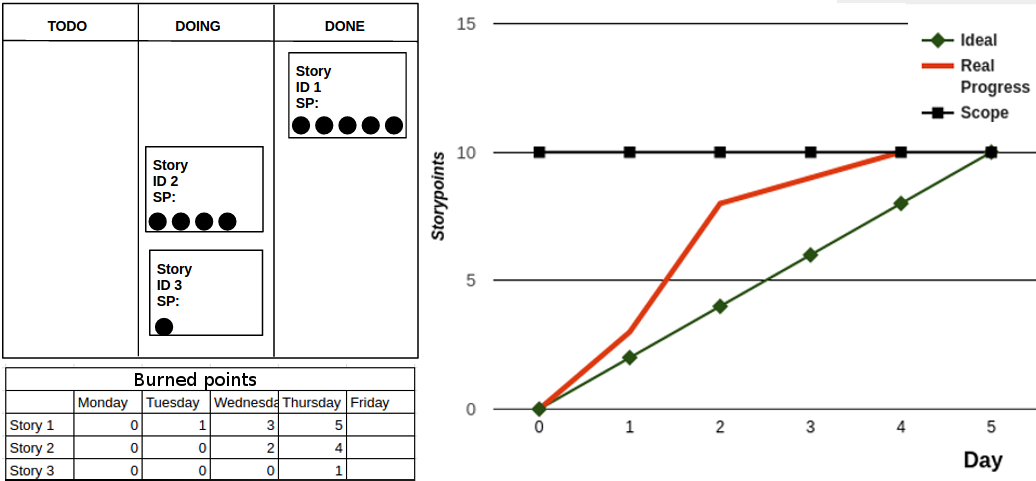
\includegraphics[width=0.90\textwidth]{Burnup-chart_example}
  \caption{Ejemplo de cómo llevar un Burnup con un sprint de 5 días y 10 puntos quemados al cuarto día.}
  \centering
  \label{fig:Burnup-chart_example} %\ref{fig:Burnup-chart_example}
\end{figure}
\FloatBarrier % Command to control the position of floating images. With its, I can get the figures not to be pushed to the end of the document.
% El comando FloatBarrier es usado aqui para que la imagen se clave en este lugar y que no sea acarreada al final del documento.

\newpage
\subsection{Gráficos de velocidad}

\subsubsection{Velocity Chart}

El gráfico de velocidad muestra todas las unidades estimadas en el plan y aceptadas (US Story Points) para un período de iteraciones realizadas\footnote{\cite{Scrum-Alliance-2014}}. También es una herramienta de monitoreo para auto-regulación ante desvíos o caídas del rendimiento y para visualizar la evolución de la capacidad de trabajo del equipo. Un gráfico de la velocidad típico, de un equipo de proyecto ágil, podría ser como el siguiente gráfico de la izquierda (ver \ref{fig:VelocityChartAndAverage}):

\begin{figure}[h]
  \centering
  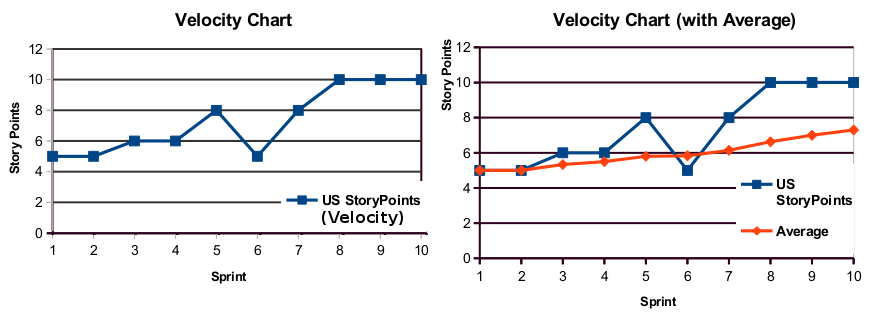
\includegraphics[width=1\textwidth]{VelocityChartAndAverage}
  \caption{Diagrama de Velocidad y Diagrama de Velocidad con Velocidad Promedio.}
  \centering
  \label{fig:VelocityChartAndAverage} %\ref{fig:VelocityChartAndAverage}
\end{figure}
\FloatBarrier % Command to control the position of floating images. With its, I can get the figures not to be pushed to the end of the document.
% El comando FloatBarrier es usado aqui para que la imagen se clave en este lugar y que no sea acarreada al final del documento.

También se puede incluir la velocidad promedio (ver gráfico de la derecha \ref{fig:VelocityChartAndAverage}).


\newpage
\section{Técnicas de programación}

Hay diferentes técnicas que pueden ser utilizadas en el proceso de desarrollo de software bajo el marco de Scrum. A continuación se describen algunas principales que sirven de soporte a metodologías ágiles:

\subsection{Técnica Pomodoro}

Se usa 'Pomodoro'\footnote{La Técnica Pomodoro es un método para la administración del tiempo desarrollado por Francesco Cirillo a fines de los años 1980\cite{Cirillo-Francesco-1980}.} como una técnica de gestión del tiempo y se basa en la hipótesis de que las pausas frecuentes en el trabajo pueden mejorar la agilidad mental. Por este motivo, la técnica consiste en dividir el tiempo dedicado a un trabajo en intervalos (time-boxing) de 25 minutos (llamados 'pomodoros') separados por descansos. Los primero tres descansos son de 5 minutos y el descanso después del cuarto pomodoro es de 15 minutos, para luego repetir la secuencia en forma cíclica. Durante el intervalo pomodoro el trabajo debe ser focalizado, por lo que no se deben admitir distracciones o trabajos ajenos al trabajo principal. 
Esta es una técnica útil en el desarrollo ágil y en la programación en pareja (pair programming) además de otros contextos de trabajo.

\begin{figure}[h]
  \centering
  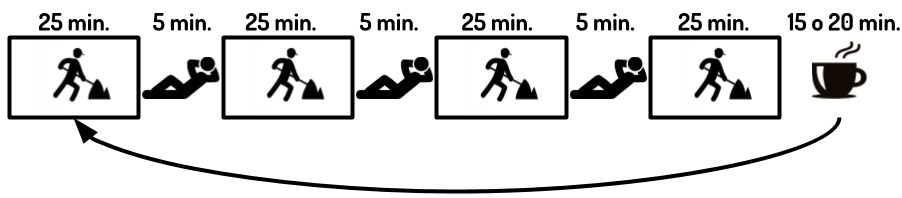
\includegraphics[width=0.80\textwidth]{Pomodoro}
  \caption{Esquema pomodoro}
  \centering
  \label{fig:Pomodoro} %\ref{fig:Pomodoro}
\end{figure}
\FloatBarrier % Command to control the position of floating images. With its, I can get the figures not to be pushed to the end of the document.
% El comando FloatBarrier es usado aqui para que la imagen se clave en este lugar y que no sea acarreada al final del documento.

\subsection{Calidad integrada}

Un programador que busca la excelencia técnica es partidario de la calidad desde el inicio o "calidad integrada", algo que en “lean manufacturing” se conoce como “quality built in”. O sea que, ser un programador ágil no es entregar rápido a expensas de la calidad y acumulando deuda técnica; ser ágil es entregar buen código, que significa que el código es legible, entendible, cubierto por test automatizado, simple y hace lo que se espera que haga. Las revisiones de código, las técnicas de TDD, los estándares de código, un DoD que contempla QA y la gestión de deuda técnica, son algunas de las prácticas que ayudan al buen código. Un buen libro que trata el tema es “Clean Code, A Handbook of Agile Software Craftsmanship” de Robert C. Martin.

\subsection{Programación de a pares}

La programación de a pares, “pairing” o “pair programming” consiste en que dos programadores participen conjuntamente en un esfuerzo combinado de desarrollo en un puesto de trabajo. La misma se puede extender al desarrollo de a pares (análisis, diseño, codificación, pruebas, diseño de interfaces de usuario, diseño gráfico, etc.).

Existen muchas razones por las que esta técnica es recomendable y las principales pueden ser las siguientes:

\begin{enumerate}

\item \textbf{Calidad:} Mejorar la calidad logrando reducir defectos por "revisión de a pares" mientras se programa.

\item \textbf{Aprendizaje:} Lograr el aprendizaje en equipo distribuyendo y nivelando el conocimiento. Pues, focalizarse en el aprendizaje es crucial para organizaciones scrum de equipos por características, donde todos deben manejar un conocimiento amplio y multidisciplinario. 

\item \textbf{Propiedad colectiva:}
Mejorar los diseños y las estimaciones debido a que todos tienen un conocimiento de la estructura del producto, un empoderamiento del mismo (propiedad colectiva del código) y de cómo puede impactar un cambio en parte de él.

\item \textbf{Resolución de problemas:} Permitir superar problemas difíciles de forma más simple, más rápido o al menos efectiva cuando trabajan juntos. La idea es que dos personas piensen mejor que una en resolver un problema.

\end{enumerate}

\subsection{Revisión de a pares}

La revisión de a pares o "peer review" es una práctica intrínseca de la actividad científica en un sistema de evaluación del trabajo científico, donde los miembros de la comunidad revisan los trabajos de sus pares\footnote{Formalmente el proceso de revisión por pares del trabajo científico fue iniciado en 1753 por la “Royal Society of London”.}. Por este motivo, implementar este tipo de prácticas en el desarrollo de software hace que sea una actividad ingenieril. El beneficio es lograr una mejor calidad y una reducción de defectos. Según Boehm "el 60 por ciento de los defectos de código se pueden eliminar durante las revisiones de a pares"\footnote{\cite{Boehm-2001}}. Así como en ciencia se revisan los trabajos de investigación antes de ser publicados, en ingeniería de software se revisa el código antes de ser desplegado.\newline
La práctica consiste en que una vez que el programador desarrolló un trabajo de codificación, solicite ante un colega compañero o un conjunto de ellos la inspección del código. Si se encuentran errores u observaciones, el desarrollador deberá mejorarlo y hasta que no tenga el visto afirmativo el código, no será desplegado o integrado al producto. Hay que tener en cuenta que para que la revisión por pares sea realmente productiva, debe ser ejecutada con el máximo de rigor, aunque implique retrasar despliegues de producto y no cumplir con los plazos comprometidos por el equipo. Cuando se aplica Scrum, el máximo de rigor incluye, además de la calidad del trabajo, prestar particular importancia al cumplimiento de la definición de terminado (DoD).

\subsection{TDD}

El "Test Driven Development" (TDD) o "desarrollo guiado por pruebas"\footnote{\cite{Jurado-2010}} es una práctica, técnica de desarrollo ágil y técnica de programación que hace foco en el comportamiento especificado de unidades de software\footnote{[Wikipedia 2014]} como disparador para el desarrollo de pruebas. O sea, basándose en especificaciones, esta práctica tiene como táctica escribir primero las pruebas (código de prueba) y después el código (código de producto) para luego realizar ciclos de "refactorización" \cite{Kent-Beck-2003}. Con este enfoque se pretende, entre otras cosas, que el diseño sea el código mismo (código de producto) y que las pruebas concretas (código de prueba) sirvan de documentación. Esta técnica se complementa con la automatización de pruebas. En todo ese conjunto de pruebas concretas, las pruebas de unidad se usan para validar métodos individuales y conjuntos de métodos. En consecuencia, en este tipo de desarrollos, se logran sistemas con un gran conjunto de pruebas (muchas líneas de código en pruebas). Por eso hay que considerar que, si bien se pueden lograr productos de calidad, demanda un costo considerable.\newline
Si tenemos que asignar un lema a este enfoque es "la prueba en primer lugar" y su afirmación filosófica principal sería que "el diseño emerge del refactoring originado por pruebas".

\subsection{Integración continua}

La integración continua (Continuous Integration\footnote{Continuous Integration fue propuesto inicialmente por Martin Fowler.}) es una práctica de ingeniería de software y modelo informático que consiste en hacer integraciones automáticas de un proyecto, compilación y ejecución de pruebas, lo más a menudo posible para así poder detectar fallos cuanto antes.

\subsection{Entrega continua}

El Continuous Delivery es un enfoque de ingeniería de software en el que los equipos producen software en ciclos cortos, garantizando releases de forma fiable en cualquier momento del desarrollo. Este modelo suele ser parte incluida en la cultura DevOps y, a su vez, suele incluir la práctica de Continuous Deployment para desplegar, en forma automática, código a producción. Trabajar bajo el marco ágil y no trabajar con testing continuo, integración continua ni entrega continua puede conducir a un trabajo poco ingenieril y menos eficiente. Es parte de reducir el time to market y el tiempo de despliegue, facilitar el flujo entre el desarrollo y despliegue, reduciéndo el tiempo lo máximo posible y manteniendo calidad. Aquí el desafío es lograr hacer el desarrollo con TDD (ATDD o DDD), integración y despliegue, todo dentro de un mismo sprint.

\begin{figure}[h]
  \centering
  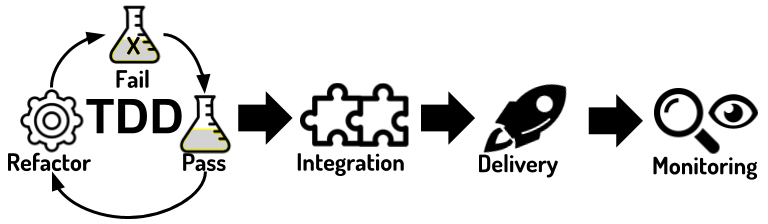
\includegraphics[width=0.80\textwidth]{Continuous_delivery_flow}
  \caption{Flujo de delivery}
  \centering
  \label{fig:Continuous_delivery_flow} %\ref{fig:Continuous_delivery_flow}
\end{figure}
\FloatBarrier % Command to control the position of floating images. With its, I can get the figures not to be pushed to the end of the document.
% El comando FloatBarrier es usado aqui para que la imagen se clave en este lugar y que no sea acarreada al final del documento.

\newpage
\section{Metodologías amigas}

El marco Scrum no es excluyente de XP, Lean, Kanban u otras metodologías. Pues, puede combinarse con cualquier otra. A Scrum se lo puede ampliar tomando aspectos de otra metodología o métodos. También se puede buscar ampliar otra metodología o métodos tomando aspectos de Scrum. Por ejemplo, se puede combinar con XP, Lean o Kanban.

\subsection{Scrum con XP}

Si hay dos sistemas ágiles de desarrollo parecidos, son Scrum y Extreme Programming. Con ambos se trabaja con iteraciones, se implementa el juego de planificación (Planning Game) o planning con el cliente o representante del negocio, se busca lograr una propiedad colectiva de código, se trata de lograr versiones pequeñas de producto para entregar rápidamente, se persigue un diseño simple, existe el rol de facilitador (Coach en XP y SM en Scrum), existe un rol que representa al cliente (On Site Customer en XP y PO en Scrum) y ambas comparten los valores de respeto y el coraje. Entre las diferencias se encuentran algunas buenas prácticas técnicas de XP y que pueden usarse bajo el marco Scrum: metáfora de sistema, pairing, continuous integration, TDD, refactoring y estándares de código. 
En mi experiencia personal, ha sido bastante común ver de la mano Scrum y XP. Aunque actualmente se ve a XP simplemente como prácticas de ingeniería de software. La construcción de un modelo mental simple del dominio del problema como metáfora al inicio del producto, en un sprint 0 o en una “inception” (incluyendo posteriormente el uso de DDD) se hace necesario para aportar más certidumbre al inicio y una guía desde donde evolucionar la estructura del sistema. El testing es crucial para construir software de calidad y TDD es una buena guía al respecto. Para desarrollar en forma incremental y evolutiva, sin acumular deuda técnica y con mejora contínua del software, es necesario practicar refactoring. Para fomentar la colaboración y la propiedad colectiva de código, la programación de a pares es útil. Para asegurar simplicidad y código claro y limpio, además de facilitar la colaboración, es que el estándar de código se usa como acuerdos de programación. Es así como en ingeniería de software con las prácticas XP se potencia a Scrum.

\subsection{Scrum con Lean}

Scrum y Lean tienen muchas coincidencias conceptuales. Para ambos, el componente humano es la piedra angular del éxito y la mejora continua una práctica fundamental. Ambos están centrados en el cliente y en entregar valor tempranamente. Más allá de esto, se puede aplicar Lean en Scrum si prestamos particular importancia a la calidad y a la reducción de los desperdicios. Un desperdicio puede ser el inventario o código acumulado sin estar operativo de cara al usuario. También los tiempos de espera o colas en cuellos de botella, tanto en actividades de desarrollo como en dependencias con otros equipos. Las comunicaciones innecesarias o gastos en comunicación burocrática. El exceso de procedimientos y protocolos corporativos. Además de la cantidad de defectos que se buscan disminuir. Las actividades que no son de valor añadido. Básicamente, añadir Lean es facilitar el flujo de trabajo, limpiandolo de los desperdicios, además de respetar los demás principios Lean. Buscar mecanismos para amplificar el aprendizaje, creando y compartiendo conocimiento. Retrasar las decisiones fundamentales, tratando de tomarlas con la mayor cantidad de información posible. Entregar valor desarrollando soluciones con integridad conceptual y cohesionadas como producto (algo que parece lógico en ingeniería de software). Y, principalmente, siempre mantener una visión global, sin encapsularse en el equipo y en soluciones locales. Esto último es prácticamente el componente de pensamiento sistémico de Lean y que el equipo puede aplicar bajo Scrum. En todo caso, de nos ser Lean usado por el equipo, tranquilamente es el SM quien puede usarlo como parte de su facilitación del proceso de trabajo.

\subsection{Ampliar Scrum con Kanban}

Scrum se puede complementar y mejorar agregando aspectos del método Kanban. Para eso se busca entregar valor con entregas tempranas y frecuentes, focalizando en hacerlo mediante un flujo de trabajo constante, estable y eficiente. Para lograrlo se siguen las siguientes reglas: 

\begin{enumerate}
\item Mostrar el proceso del flujo de trabajo.
\item Limitar el trabajo en curso (WIP). 
\item Optimizar el flujo.
\item Inspeccionar y adaptar las “reglas de juego”.
\end{enumerate}

Para mostrar el proceso hay que reemplazar en el tablero kanban los estados ambiguos o genéricos por concretos, como por ejemplo el estado “en progreso” (“on going” o “doing”) por todos los estados reales del flujo de trabajo en curso.  Un ejemplo de un flujo completo (ver fig. \ref{fig:Scrum-Kanban-Board-to-Development}) puede ser: nueva (new), refinanda (refining), lista (ready), comprometida (committed), desarrollando (developming), probando (testing), completa (done), aceptada (accepted), desplegando (deploy) y en operación (operative). Hecho esto, el equipo debe buscar mantener el foco de trabajo del sprint en un límite de cantidad de historias que se trabajan en paralelo (WIP). El equipo debe buscar descubrir cuál es el límite con el que pueden trabajar con cadencia sin peligrar el objetivo del sprint. Debe buscar que no hayan cuellos de botella en ninguno de estos estados o pasos del flujo. Y, finalmente, revisar y mejorar constantemente sus reglas de juego: DoR, DoD, acuerdos de trabajo, nomenclaturas de los tableros kanban y hasta el marco de trabajo mismo.

Esto es lo básico que se debería hacer para sumar el método Kanban a Scrum. Desde un punto de vista, prácticamente sistémico y Lean, un SM debe pensar a su equipo como si fuera un sistema a estabilizar y facilitar la maximización de su flujo de trabajo. El SM debería ser también una especie de “Flow Master”, un facilitador del flujo. Es así que también se pueden agregar el manejo de las métricas Kanban, como el cycle time y throughput (o delivery rate), y herramientas de monitoreo visual como el diagrama de flujo acumulado o CFD.

\begin{figure}[h]
  \centering
  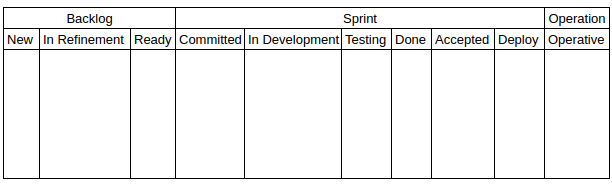
\includegraphics[width=1\textwidth]{Scrum-Kanban-Board-to-Development}
  \caption{Tablero Scrum-Kanban ejemplo para un equipo de desarrollo}
  \centering
  \label{fig:Scrum-Kanban-Board-to-Development} %\ref{fig:Scrum-Kanban-Board-to-Development}
\end{figure}
\FloatBarrier % Command to control the position of floating images. With its, I can get the figures not to be pushed to the end of the document.
% El comando FloatBarrier es usado aqui para que la imagen se clave en este lugar y que no sea acarreada al final del documento.

\subsection{Ampliar Kanban con Scrum, Scrumban}

Una metodología amiga de Scrum es Scrumban. Se trata de una pseudo-metodología mixta y flexible entre Scrum y el método Kanban. Combina las la flexibilidad de Kanban y las características básicas de Scrum. Por un lado, se toma de Kanban lo de mantener un trabajo continuo, exponer el flujo de trabajo, el tablero de trabajo persistente, auto-asignaciones de tareas solamente por el sistema del tomar y jalar (pull), limitar el trabajo en curso y buscar optimizar el flujo teniendo en cuenta la métrica “cycle time”. Por otro, se agrega de Scrum la ceremonia de planning, la retrospectiva como reunión de mejora contínua (Kaizen), el trabajo en ciclos o iteraciones sin ser limitativo o restrictivo de trabajo y la priorización, que se recomienda hacer en cada planificación. Dentro de la flexibilidad que brinda, hace optativo el usar otras partes o prácticas de Scrum. Bajo esta metodología no es necesario estimar, puede ser algo optativo, ya que no se necesita calcular el trabajo que entra en una iteración porque el trabajo es continuo. Aunque sí se pueden estimar tiempos de entrega y/o tamaños de paquetes de trabajo. Por otro lado, al ser el trabajo contínuo y no tener un compromiso formal de trabajo comprometido en una iteración, los cambios y re-priorizaciones pueden hacerse en cualquier momento. 
 
También es muy flexible el tipo de roles de los miembros del equipo debido a que no prescribe roles específicos ni es necesaria la multidisciplinariedad que recomienda Scrum. Sin embargo en los equipos Kanban o Scrumban han emergido las figuras de Product Owner y Flow Master (facilitador equivalente a un Scrum Master). En Scrumban el Flow Master es, además de un facilitador ágil, un facilitador del flujo del proceso. Usando la facilitación visual hay que tener en cuenta que, como se mencionó antes y al igual que en Kanban, el tablero permanece persistente, mientras que sólo cambian las tareas y sus prioridades. A diferencia de Scrum, donde el tablero de sprint se renueva en cada iteración. Relacionado a la planificación, en Scrumban se planifica focalizados en los releases y no es obligadamente necesario hacerse en la planning de cada iteración; pues, la planificación se puede realizar solo bajo demanda. Este método es muy útil principalmente para procesos de ritmo rápido, para startups, proyectos que requieren fabricación de productos constante, equipos y proyectos con ambientes muy dinámicos y cambiantes, equipos de solución de problemas de contingencias en producción, equipos de mantenimiento, soporte o desarrollo de infraestructura. También es útil para integrar (coordinar y sincronizar) otros equipos de soporte a los equipos Scrum, por ejemplo bajo el marco DevOps. En estos casos, los equipos soporte pueden usar Scrumban y los de desarrollo Scrum.

\begin{figure}[h]
  \centering
  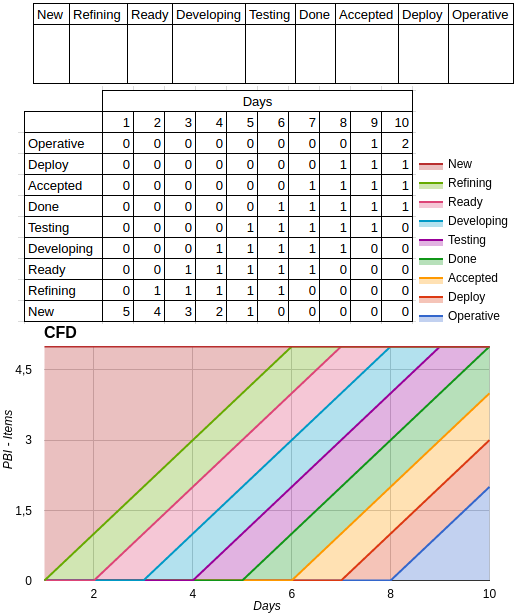
\includegraphics[width=0.80\textwidth]{Scrumban-Board-to-Development}
  \caption{Tablero Scrumban y CFD ejemplo para un equipo de desarrollo}
  \centering
  \label{fig:Scrumban-Board-to-Development} %\ref{fig:Scrumban-Board-to-Development}
\end{figure}
\FloatBarrier % Command to control the position of floating images. With its, I can get the figures not to be pushed to the end of the document.
% El comando FloatBarrier es usado aqui para que la imagen se clave en este lugar y que no sea acarreada al final del documento.
